\chapter{Flight Controller Design}\label{ch:sw}
The flight controller developed is a control structure for stabilization of a quad-rotor. The flight controller takes data from different sensors to get the position and orientation of the drone and uses a Proportional Integral and Derivative (PID) control to stabilize the drone. It is developed is based on the YMFC-AL and YMFC-32 projects by Joop Brokking \cite{bib:brooking}, where the author develops a fight controller for an Arduino Uno and STM32 board. This project was translated to C language and configured to work with De10-Nano with necessary libraries \cite{bib:gpsLib} \cite{bib:tu_viena}.
The fight-controller developed has multiple functionalities apart from stabilization and this requires a 6-channel transmitter to switch to different modes. Channel 1-4 are used to control the quad copter movements which are throttle, roll, pitch and yaw respectively. Channel 6 is used lock heading of the drone to one direction also known as holonomic motion. Whereas the channel 5 is used to control the mode of flight which are:
\begin{itemize}
    \item Manual mode- for 0-1200 pulse width 
    \item Altitude hold mode- for 1200-1600 pulse width 
    \item Position hold mode- for 1600-1950 pulse width 
    \item Return To Home- for greater than 1950 pulse width
\end{itemize}
These modes are further explained in detail in Sec. \ref{sec:general_working}.
The above defined modes are possible by receiving different data from different sensors attached to the drone such as:
\begin{itemize}
    \item Inertial Measurement Unit (IMU) - to provide the drone's orientation data i.e. the pitch, roll and yaw angles
    \item Barometer - To provide the altitude at which the drone is flying
    \item Global Positioning System (GPS)- to provide the global positioning of the drone
    \item Compass - to provide the absolute heading of the drone.
    \item Telemetry - To send and receive data from the drone during its flight
    \item ADC module - To convert battery voltage to digital values for drone stabilization
    \item FTDI -  To upload a program to the FPGA board.
    \item Electronic Speed Controller (ESC) - It is used to control the brushless DC motors using PWM signals
\end{itemize}

\section{General Working}\label{sec:general_working}
The flight controller works on a multi-core architecture with 4 parallel cores, where the PID controller, LED devices and analog read run on main core which is core-0; the I2C devices like, compass, IMU, Barometer run on core-1; the PWM signals devices like ESCs and RF- receiver are in core-2; the UART devices like GPS and Telemetry are in core-3. All the cores run at 50Hz whereas the GPS runs are a slower speed due to time it takes to read the data.

The Flight controller program receives the orientation data from IMU and compass, altitude data from Barometer, position data from GPS, Battery voltage from analog pins of the FPGA. The data from IMU, barometer, compass and GPS are provided as feedback to the PID controller, which controls the drone in different modes. Additionally, the supplied voltage from the battery decreases overtime during the flight of the drone. To compensate this, the battery voltage is read from the ADC module and it is used to correct the output for the motors as seen from Fig. \ref{fig:flight_controller}. A test code for battery voltage calculator module was developed \ref{ch:test}, but this functionality was not implemented together with the final version of the flight controller code due to time constraints.

\begin{figure} [H]
    \centering
    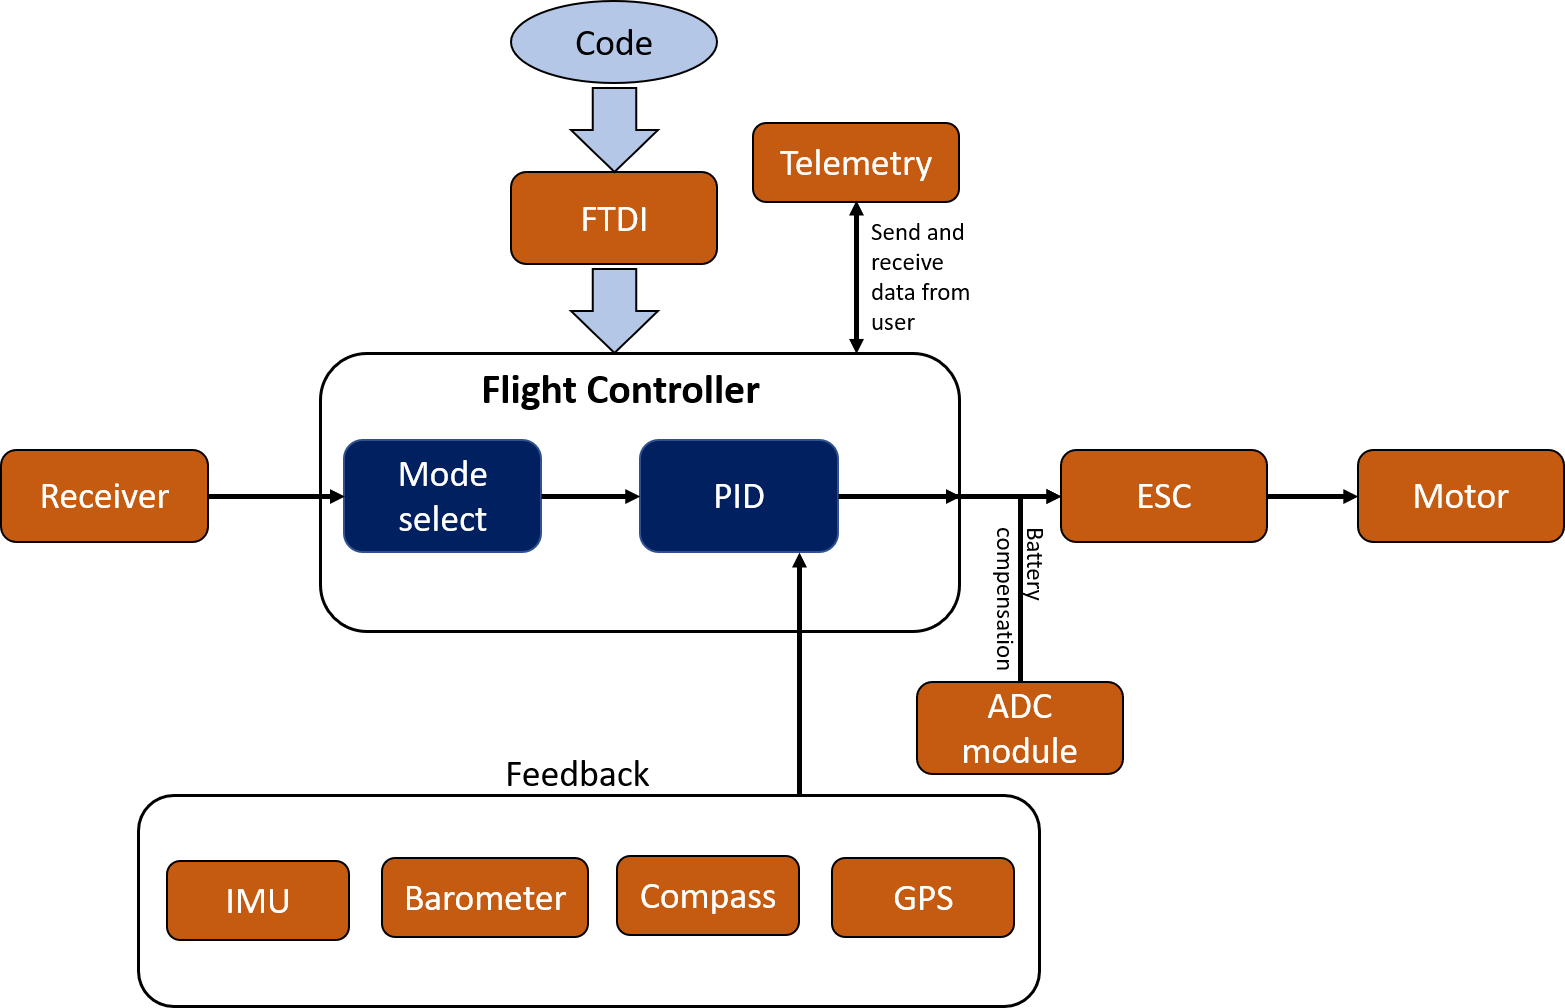
\includegraphics[width=\textwidth]{Figures/implementation/flight_controller.png}
    \caption{Overview of Flight controller model}
    \label{fig:flight_controller}
\end{figure}

Working of different modes:
\subsection{Manual mode}\label{subsec:manual_control}
Manual mode is used to navigate the drone using a transmitter controlled by a pilot. It is achieved only by using an IMU. The controller calculates the motor pwm signals based on the input from the IMU and the RF-transmitter. This is then fed to the esc of the respective motors to control the pitch, roll and yaw of the drone. This functionality has been tested and is its PID gains are fined tuned for stabilization.
\subsection{Altitude hold}\label{subsec:altitude_hold}
Altitude hold mode is to make the drone hover at a constant altitude. This mode is achieved using an IMU and a barometer, where the IMU does the same functions as mentioned in Sub-section \ref{subsec:manual_control} and barometer data is used to control the throttle of all the motors to achieve altitude stabilization. This functionality was tested to output proper results, but the PID gains were not properly tuned due to time constraints.
\subsection{Position hold}\label{subsec:position_hold}
Position hold mode is to make the drone hover and stay fixed at a certain position provided. This mode is achieved using an IMU, compass, barometer and a GPS, where the GPS and compass, provides the position and absolute heading information of the drone and this is used to control the drone to remain at a fixed position. This functionality has not been tested due to low frequency of GPS data, and issues regarding core-3 hanging. Information regarding core-3 issues is explained in Chapter \ref{ch:concl}.
\subsection{Return To Home}\label{subsec:rth}
The drone records the home position at the beginning and when this mode is switched on, it return back to the recorded home location. This mode also, uses IMU, compass, Barometer and GPS to achieve this task. Similarly, due to the issues regarding core-3, this functionality has not been tested.
























